\documentclass[a4paper,12pt,titlepage]{article}
\usepackage[utf8]{inputenc}
\usepackage{graphicx} % Required for inserting images
\usepackage[spanish,es-tabla]{babel}
\usepackage[none]{hyphenat}
\usepackage[justification=centering]{caption}
\usepackage{subcaption}
\usepackage{amssymb, amsmath}
\usepackage{gensymb}
\usepackage{fancyhdr}
\usepackage{wrapfig}
\usepackage{physics}

\usepackage[a4paper]{geometry}
\geometry{top=3cm, bottom=3.0cm,left=2cm, right=2cm}


\lhead{ELV binario}
\rhead{Gonzalo Bastos González}

\pagestyle{fancy}

\title{Equilibrio líquido-vapor en sistemas binarios}
\author{Gonzalo Bastos González}
\date{Técnicas expermimentales II-Laboratorio de termodinámica}

\begin{document}

\maketitle
\tableofcontents

\newpage

\section{Objetivos e introducción teórica}

El objetivo de esta práctica es estudiar la curva de condensación-ebullición del sistema binario formado por agua y etanol. Para un estudio más completo calcularemos los coeficientes de actividad en fase líquida de los dos componentes de la mezcla así como la entalpía libre de exceso de la mezcla.

\begin{figure}[h!]
    \centering
    \begin{subfigure}{0.45\textwidth}
        \centering
        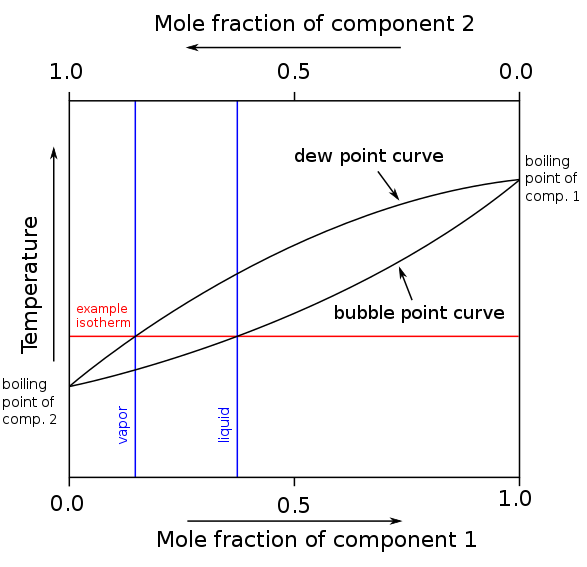
\includegraphics[width=0.85\linewidth]{ELV binario/curva_cond.png}
    \end{subfigure}
    \begin{subfigure}{0.45\textwidth}
        \centering
        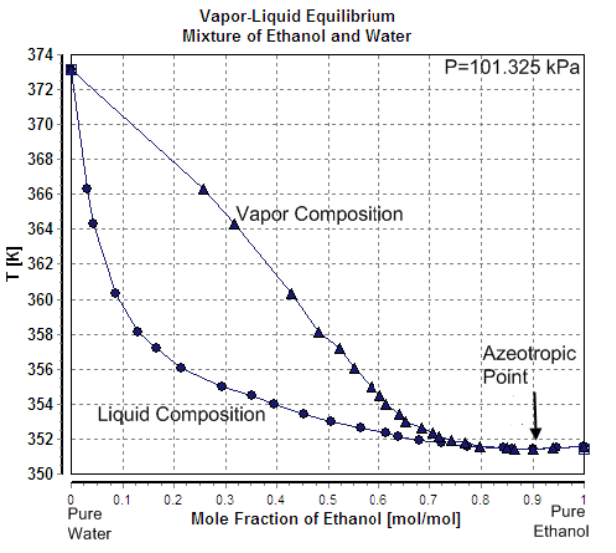
\includegraphics[width=0.85\linewidth]{ELV binario/curva_cond2.png}
    \end{subfigure}
    \caption{Ejemplos de curvas de condensación ebullición}
\end{figure}

Para el estudio de nuestro sistema necesitamos ciertas variables que lo caractericen, para un sistema binario las variables a emplear son $(T,p,n_1,n_2)$. No obstante, nuestro sistema se puede considerar cerrado, lo que da lugar a la ligadura $n_1+n_2 = n_t = cte.$Por tanto, solo necesitamos tres variables para caracterizar nuestro sistema, $(T,p,n_i)$, o si dividimos entre los moles totales para emplear la fracción molar $(T,p,\chi_i)$. Durante nuestra práctica trabajaremos en un ebullómetro a presión constante, por lo que las únicas variables que manejaremos son la presión y la fracción molar, que nos permitirán caracterizar las curvas de coexistencia como $T=T(\chi_i)$.

En nuestras curva de coexistencia de ejemplo podemos ver que existen dos curvas, la curva del etanol y la curva del agua. Esto se debe a que el etanol presenta una temperatura de ebullición mucho más baja que la del agua, por lo que siempre existe un rango de temperaturas en el que coexisten la fase líquida y vapor de ambas sustancias. En el caso real estas curvas coinciden en un único punto, el punto azeotrópico, donde la concentración de uno de los componentes se acerca a cero.

Otra de las magnitudes que caracterizan los sistemas multicomponente son los potenciales químicos:

\begin{equation}
    \mu_i = \mu_i^0 + RT\ln \chi_i
\end{equation}

Donde $R$ es la constante de los gases ideales y $\mu_i^0$ es el potencial químico del estado de referencia. Esta magnitud se define así para sistemas ideales, para sistemas reales se define el concepto de actividad del componente, $a_i$, que es aquella magnitud que verifica:

\begin{equation}
    \mu_i = \mu_i^0 + RT \ln a_i = \mu_i^0 + RT \ln \chi_i \gamma_i
\end{equation}

Donde $\gamma_i = a_i/\chi_i$ es el coeficiente de actividad, que mide la desviación de la idealidad del componente $i$. Para un componente ideal $\gamma_i=1$, la actividad coincide con la fracción molar. El coeficiente de actividad para nuestra mezcla agua-etanol, suponiendo una fase vapor ideal, de las componentes en fase líquida se puede expresar como:

\begin{equation}
    \gamma_i^l (T) = \frac{\chi_i^v (T) p}{\chi_i^l(T)p_i^0(T)}
    \label{gamma}
\end{equation}

Donde los superíndices $l$ y $v$ hacen referencia a la fase líquida y vapor respectivamente, $p$ es la presión del laboratorio y $p_i^0$ es la presión de equilibrio líquido-vapor\footnote{Se obtiene a partir de los datos de la práctica ELV simple} del componente $i$ en estado puro a la temperatura T. La incertidumbre de los coeficientes de actividad se puede obtener por propagación a partir de la siguiente expresión:

\begin{equation}
    s(\gamma^l_i (T)) = \frac{\chi^v_i}{\chi^l_i p_i^0} \sqrt{ s(\chi_i^v)^2 + \left( \frac{\chi_i^v}{\chi_i^l} \right)^2 s(\chi_i^l)^2 + \left(\frac{\chi_i^v}{p_i^0}\right)^2 s(p_i^0)^2}
    \label{inc_gamma}
\end{equation}

Otra magnitud interesante de estudiar es la entalpía libre molar de exceso $\Delta g^{E}$, que nos da la diferencia entre la entalpía libre de mezcla del sistema no ideal $\Delta g^M$ y la del ideal $\Delta g^{M,id}$:

\begin{equation}
    \begin{gathered}
    \Delta g^{E} = \Delta g^M - \Delta g^{M,id} = RT \sum_i \chi_i \ln a_i - RT \sum_i \chi_i \ln \chi_i = RT \sum_i \chi_i^l \ln \gamma_i^l \\
    \Delta g^{E} = RT (\chi_{H_2O}^l \ln \gamma_{H_2O}^l + \chi_{OH}^l \ln \gamma_{OH}^l )
    \end{gathered}
    \label{delta_g}
\end{equation}

La incertidumbre de la entalpía libre de exceso se puede obtener aplicando propagación de incertidumbres a la expresión anterior:

\begin{equation}
    s(\Delta g^{E}) = RT \sqrt{ \left( \sum_i (\chi_i^l \ln \gamma_i^l) \right)^2 \left( \frac{s(T)}{T} \right)^2 + \sum_i \left(\ln \gamma_i^l s(\chi_i^l)\right)^2 +\sum_i \left( \frac{\chi_i^ls(\gamma_i^l)}{\gamma_i^l} \right)^2}
\end{equation}

Donde los subíndices $i$ hacen referencia a los dos componentes de nuestro sistema termodinámico que debemos tener en cuenta durante el cálculo de las incertidumbres, $i=OH,H_2O$.

Por último, vamos a abordar la idealidad de nuestro sistema de otra forma, empleando la ley de Raoult, que establece una relación entre la presión parcial de un componente $p_i$, su fracción molar $\chi_i$ y su presión de vapor $p_i^0$ en una disolución

\begin{equation}
    p_i =\chi_i^l p_i^0  
\end{equation}

Además de eso en un sistema ideal se verifica la ley de Dalton, que dice que la presión total es la suma de las presiones parciales:

\begin{equation}
    p = \sum_i p_i
\end{equation}

Por tanto, combinando la ley de Raoult con la ley de Dalton podemos obtener la siguiente expresión para la presión total de la disolución:

\begin{equation}
    p^R = \sum_i \chi_i^l p_i^0
\end{equation}

Donde $p^R$ hace referencia a la presión ideal predicha por la ley de Raoult, que compararemos con la presión del laboratorio para estudiar la desviación de la idealidad de nuestro sistema. Para obtener la incertidumbre de la presión de Raoult vamos a aplicar propagación de incertidumbres a la expresión anterior:

\begin{equation}
    s(p^R) = \sqrt{ \sum_i \left(p_i^0 s(\chi_i^l)\right)^2  + \sum_i \left(\chi_i^l s(p_i^0)\right)^2} \quad i=OH,H_2O
\end{equation}

\section{Materiales y metodología}

Para realizar nuestra práctica contamos con un ebullómetro en el laboratorio, que cuenta con los siguientes componentes

\begin{itemize}
    \item Matraz esférico (1) en el que se encontrará el equilibrio líquido-vapor de etanol y agua. Cuenta con un conducto que emplearemos para contaminar el sistema con agua o etanol.
    \item Resistencia conectada (2) a un generador de corriente para calentar el sistema.
    \item Sistema de refrigeración (3), cuando la fase líquida comienza a hervir pasa por una serie de tubos que se encuentran en contacto con agua fría del grifo que harán que la mezcla condense y pase de nuevo al matraz a través de un sistema de reciclado de vapor.
    \item Válvulas de extracción (4,5), para tomar muestras de la fase líquida y vapor que extraeremos en frascos para su posterior estudio.
    \item Sonda (6) conectada a un medidor de temperatura digital externo para medir la temperatura de ebullición en cada instante.
    \item Baño de calor para mantener las muestras a una temperatura controlada.
    \item Densímetro digital.
\end{itemize}

\begin{figure}[h!]
    \centering
    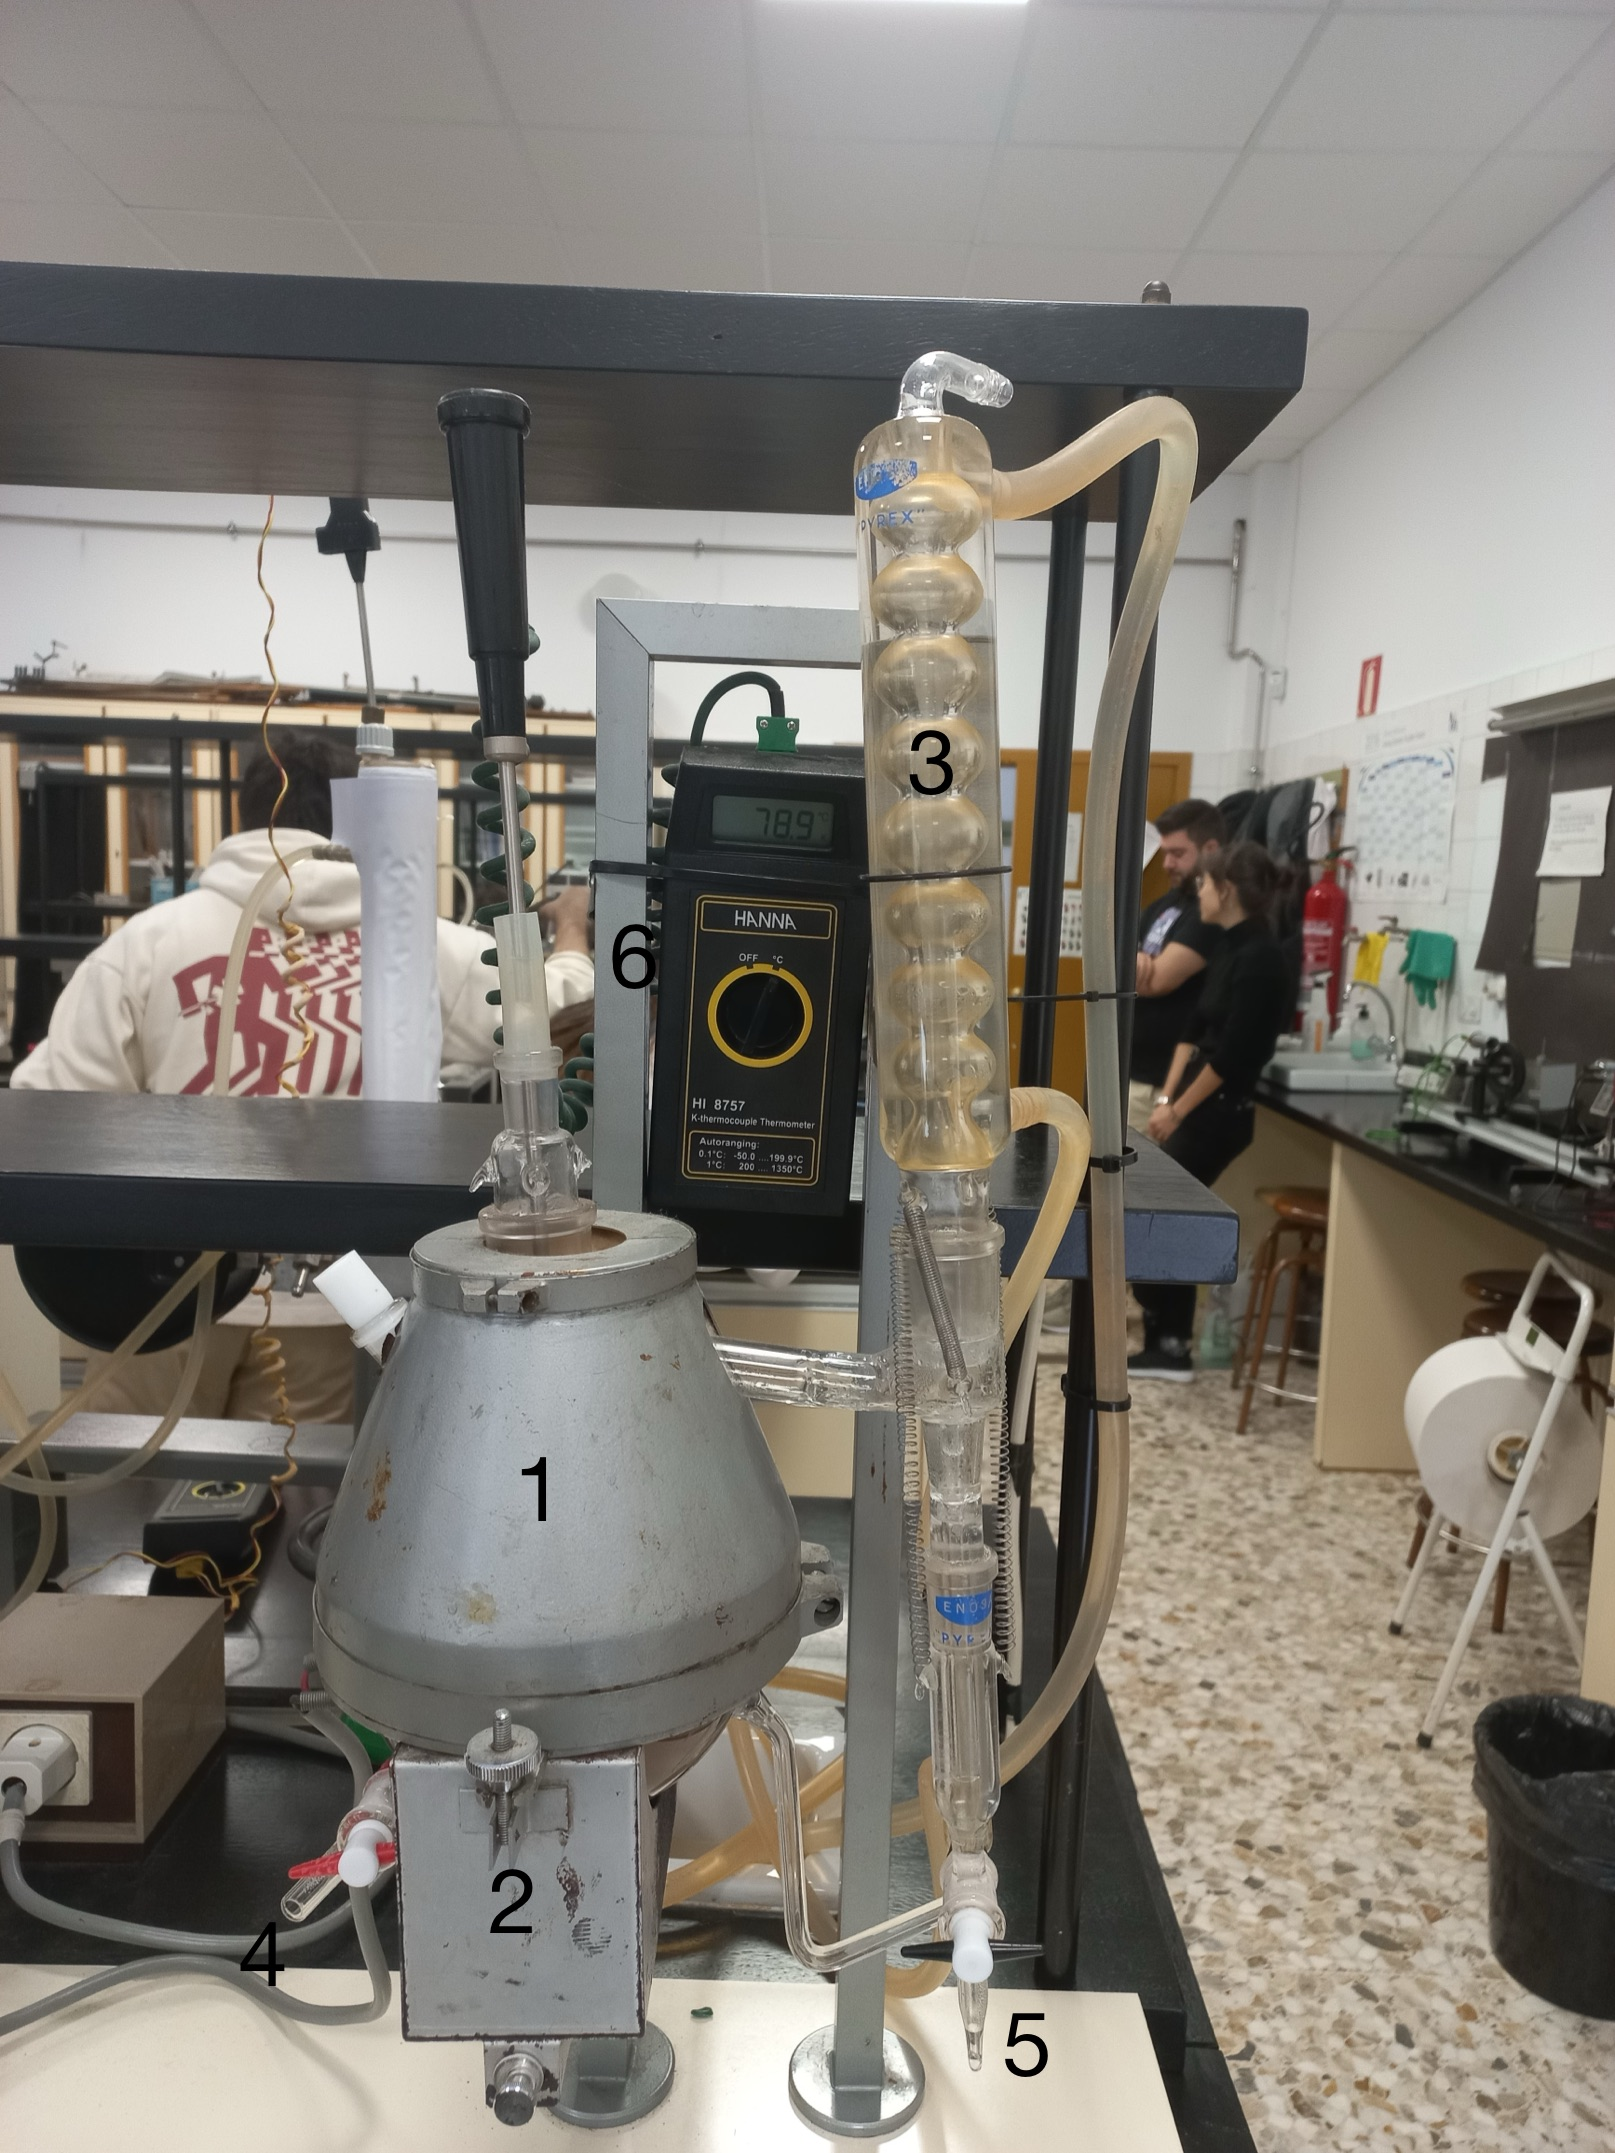
\includegraphics[width=0.55\linewidth]{ELV binario/ebullometro.jpg}
    \caption{Ebullómetro empleado en el laboratorio}
    \label{fig:enter-label}
\end{figure}

El procedimiento experimental llevado a cabo es muy sencillo, partimos del matraz lleno de uno de los dos componentes, agua o etanol y contaminaremos el sistema con el otro componente para crear un sistema binario de etanol y agua cuya fracción molar de los componentes iremos variando. La primera serie de medidas parte del matraz lleno de agua, por lo que la temperatura a la que se encontrará inicialmente es la temperatura de ebullición del agua. Una vez tengamos nuestro sistema en equilibrio, es decir la temperatura esté fija y la fase vapor esté entrando de nuevo en el matraz por el sistema de recuperación procederemos a retirar muestras de fase líquida y vapor, unos 15 mL de cada una que introduciremos en el baño de calor para su posterior estudio. Después de retirar las muestras introduciremos 30 mL de etanol en el matraz para mantener el volumen más o menos constante. Cuando la temperatura el sistema vuelva de nuevo al equilibrio repetiremos de nuevo el proceso de extracción de muestras, reduciendo así la temperatura de ebullición a medida que añadimos más etanol, que tiene una temperatura de ebullición menor. Repetiremos este proceso hasta que la temperatura de ebullición alcance unos $84^{\circ} C$, temperatura a la que finalizaremos la primera toma de medidas.

Para la segunda toma de medidas el procedimiento será exactamente igual, salvo que en esta ocasión partimos de un matraz lleno de etanol al que iremos añadiendo agua destilada. En esta ocasión, a medida que vamos tomando muestras y añadiendo agua destilada vemos como la temperatura de ebullición va aumentando, ya que, como hemos mencionado antes, la temperatura de ebullición del agua es mayor que la del etanol. La segunda toma de muestras finalizará cuando la temperatura de ebullición llegue a la temperatura a la que finalizamos la serie anterior, para tener así una curva completa.

La otra parte del trabajo de laboratorio consiste en el estudio de las muestras extraídas del ebullómetro, de fase líquida y vapor. La magnitud que nos permite caracterizar la composición de cada muestra es su densidad, que podemos medir con nuestro densímetro digital. Para ello partiremos de la expresión analítica de $\rho(\chi)$ obtenida durante la práctica de densidad, que invertiremos para obtener una expresión para $\chi(\rho)$ que nos permitirá caracterizar las curvas de condensación-ebullición. El densímetro nos permite obtener pares de valores $(\rho,T)$, que se miden de forma directa al introducir la muestra con una jeringuilla en el aparato. La incertidumbre de estas magnitudes viene dada por la precisión del propio densímetro:

\begin{equation}
    s(\rho) = 0,0001 \;g/cm^{3} \quad s(T)=0,1 \; ^{\circ}C
\end{equation}

\subsection{Cálculos previos}

Como ya hemos avanzado antes, necesitamos datos de otras prácticas realizadas anteriormente. En concreto, de la práctica de densidad en sistemas binario necesitamos el ajuste $\rho(\chi)$ antes mencionado y de la práctica de equilibrio líquido-vapor simple las presiones de equilibrio de las sustancias puras.

\subsubsection{Expresión analítica de $\chi(\rho)$}

A partir de los datos de $\rho(\chi_{H_2O},T)$ tomados durante la práctica escogemos una isoterma sobre la que trabajar, en nuestro caso de $28^{\circ}$, la temperatura de trabajo. Con los datos de la isoterma tenemos una serie de medidas de $\rho(\chi)$ que podemos buscar ajustar a alguna función. En nuestro caso elegimos un ajuste a un polinomio de segundo grado, de la forma $\rho(\chi) = a\chi^2 + b\chi + c$. Escogimos esta forma funcional porque es especialmente útil para obtener su inversa, la función $\chi(\rho)$ que necesitamos para esta práctica, que se puede calcular con la fórmula de Bhaskara:

\begin{equation}
    \rho = a\chi^2 + b\chi + c \Rightarrow \chi = \frac{-b + \sqrt{b^2 - 4a(c-\rho)}}{2a}
    \label{chi_rho}
\end{equation}

Cabe destacar que solo tomamos la solución positiva de la ecuación, pues la solución negativa no tiene sentido físico, ya que da valores negativos de la fracción molar. A partir de esta ecuación podemos obtener la incertidumbre de $\chi$ por propagación:

\begin{equation}
    \begin{gathered}
        s(\chi) = \sqrt{ \left( \frac{b-k}{2a^2} + \frac{2(\rho - c)}{ka} \right)^2 s(a)^2 + \left(\frac{b}{2ka} - \frac{1}{2a} \right)s(b)^2 + \left( \frac{s(c)}{k} \right)^2 + \left( \frac{s(\rho)}{k} \right)^2} 
        \\
        k \equiv \sqrt{b^2 - 4a(c-\rho)}
    \end{gathered}
\end{equation}

A partir de esta expresión queda claro que la incertidumbre de las fracciones molares van a depender de la densidad, no se van a mantener constantes. A partir de estas expresiones tendremos $\chi \pm s(\chi)$ para poder construir las curvas de coexistencia de $T_{eb}$ frente a  $\chi_{H_2O}$. Los parámetros empleados, obtenidos a partir del ajuste $\rho(\chi)$ son:

\begin{table}[h!]
    \centering
    \begin{tabular}{|c|c|}
    \hline
    $a \pm s(a) \;(g/cm^3)$ & $0,1516 \pm 0,0091$ \\ \hline
    $b\pm s(b) \; (g/cm^3)$ &  $0,047 \pm 0,010$\\ \hline
    $c \pm s(c) \; (g/cm^3)$ & $0,7971 \pm 0,0025$\\ \hline
    \end{tabular}
    \caption{Datos del ajuste $\rho(\chi)$}
    \label{tab:my_label}
\end{table}

No obstante, debemos destacar que para construir este polinomio no pudimos emplear totalmente nuestros datos de la práctica de densidades, pues obtuvimos valores extrañamente altos las densidades correspondientes a fracciones molares bajas de agua, lo que daba lugar a resultados poco coherentes a la hora de calcular las curvas de coexistencia, como por ejemplo la falta de puntos azeotrópicos. Para ello sustituimos las densidades anómalas de las últimas fracciones molares de agua por datos de otros compañeros que emplearon el mismo densímetro, obteniendo un resultado mucho mejor para el polinomio de $\rho(\chi)$.

\subsubsection{Presiones de equilibrio de las sustancias puras}

Otra expresión necesaria para el desarrollo de la práctica es la relación entre la presión en función de la temperatura para las sustancias puras en una situación de equilibrio líquido-vapor. Para ello vamos a recurrir a los datos de la práctica de \textit{ELV simple}, donde a partir de medidas de presión y temperatura obtuvimos la siguiente relación:

\begin{equation}
    \ln p = cte - \frac{l^v}{R}\frac{1}{T}
    \label{ln p}
\end{equation}

Si aplicamos exponenciales a ambos lados de la ecuación podemos obtener una expresión analítica para $p(T)$, que coincide con la ecuación de la curva de coexistencia. A partir de esta expresión durante la práctica realizamos un ajuste exponencial a una función del tipo:

\begin{equation}
    p = ce^{b/T}
\end{equation}

Donde $c$ es la constante de integración, que se podría calcular con un punto de referencia $(p_0,T_0)$, pero nosotros vamos a estimar con nuestro ajuste. Por convención, de aquí en adelante vamos a denominar este término como $p_0$. Por otro lado, el otro parámetro $b$ se relaciona directamente con los calores de vaporización de las substancias, como se demuestra en esa práctica. Por tanto, la expresión final de $p(T)$ tiene la siguiente forma:

\begin{equation}
    p(T) = p_0 e^{-l^v/RT}
\end{equation}

Los parámetros empleados para los ajustes son los de las regresiones exponenciales, que presentan mejores resultados que las lineales. Además de eso consideraremos las series de medidas en las que subía la temperatura, ya que presentaban valores de $l^v$ más próximos a los valores de referencia que consideramos durante esa práctica. En la siguiente tabla podemos ver los parámetros empleados:

\begin{table}[h!]
\centering
\begin{tabular}{c|c|c|}
\cline{2-3}
                & Etanol & Agua \\ \hline
\multicolumn{1}{|c|}{$p_0 \pm s(p_0) \;(Pa)$}     & $(1,030 \pm 0,031) \cdot 10^{11}$  & $(3,825 \pm 0,077) \cdot 10^{10}$  \\ \hline
\multicolumn{1}{|c|}{$l^v \pm s(l^v) \; (J/mol)$} & $40474 \pm 96$ & $39712 \pm 69$ \\ \hline
\multicolumn{1}{|c|}{$l^v \pm s(l^v) \; (kJ/kg)$} & $878,6 \pm 2,1$ &  $2206,2 \pm 3,8$    \\ \hline
\end{tabular}
\caption{Parámetros de las ecuaciones $p(T)$}
\label{tab:my-table}
\end{table}

En la siguiente figura podemos ver una representación gráfica de los datos experimentales empleados, así como los resultados de los ajustes exponenciales:

\newpage

\begin{figure}[h!]
    \centering
    \begin{subfigure}{0.49\textwidth}
        \centering
        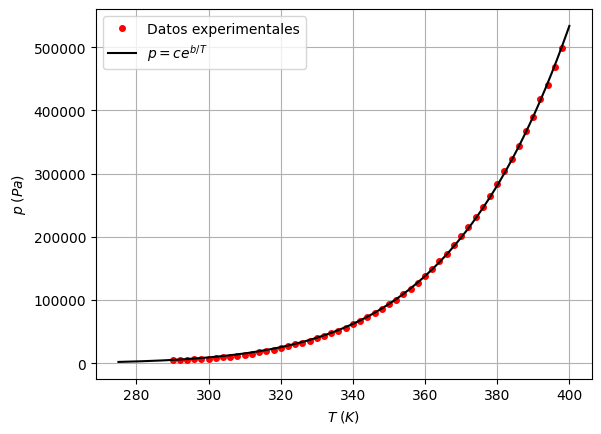
\includegraphics[width=1.02\linewidth]{ELV simple/curva_c_oh.png}
        \subcaption{Etanol}
    \end{subfigure}
    \begin{subfigure}{0.49\textwidth}
        \centering
        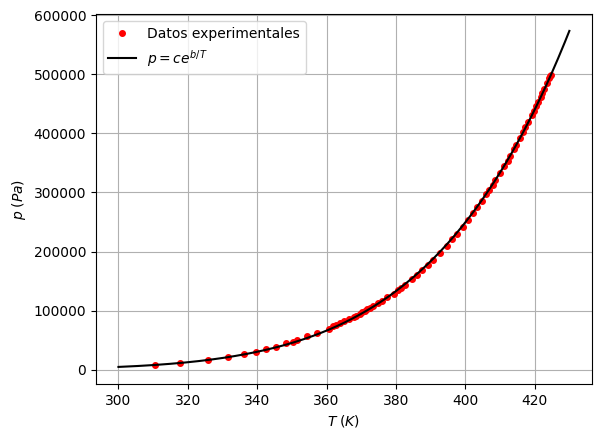
\includegraphics[width=1.02\linewidth]{ELV simple/curva_c_agua.png}
        \subcaption{Agua}
    \end{subfigure}
    \caption{Datos experimentales y ajuste $p=p_0e^{-l^v/RT}$}
    \label{fig:enter-label}
\end{figure}

Para obtener una expresión para la incertidumbre de $p(T)$ no tenemos más que aplicar propagación de incertidumbres a la expresión anterior:

\begin{equation}
    s(p) = e^{-l^v/RT} \sqrt{s(p_0)^2 + \left( \frac{p_0}{RT} \right)^2 s(l^v)^2 + \left( \frac{p_0 l^v}{RT^2} \right)^2 s(T)^2}
\end{equation}


\section{Resultados experimentales y tratamiento de datos}

\subsection{Curvas de coexistencia}

Como ya hemos mencionado anteriormente, el procedimiento experimental se basa en el estudio de la temperatura de ebullición y como varía esta en función de la composición del sistema. Las medidas de la densidad de la fase líquida y la fase vapor nos permiten obtener la fracción molar de cada componente en esa muestra a partir de la expresión $\chi(\rho)$. Una vez tengamos estos valores ya podemos obtener las curvas de coexistencia representando la temperatura de ebullición, $T_{eb}$, frente a la fracción molar de uno de los componentes, en nuestro caso tomamos como referencia la fracción molar del agua. En la tabla que figura en el anexo podemos ver los datos experimentales tomados en el laboratorio de las dos fases, así como la temperatura de ebullición a la que corresponden.

A partir de estos datos experimentales, empleando la Ec.\ref{chi_rho}, podemos obtener las curvas de coexistencia de las fases líquida y vapor, que se puede ver en la siguiente figura.

\begin{figure}[h!]
    \centering
    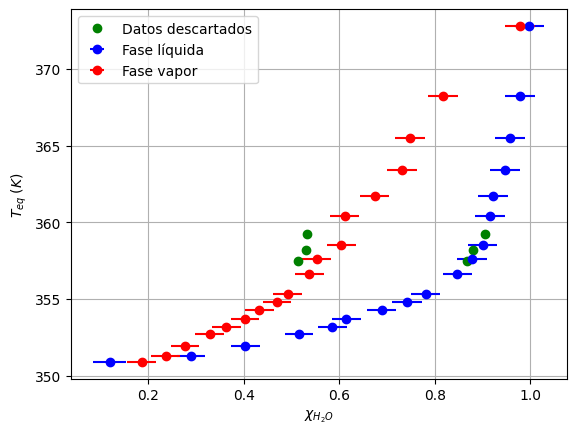
\includegraphics[width=0.65\linewidth]{ELV binario/curva_descartes.png}
    \caption{Curvas de coexistencia líquido-vapor para el sistema etanol-agua}
    \label{fig:enter-label}
\end{figure}

En la gráfica se aprecian tres datos anómalos en la curva del vapor, datos van a ser descartados, algo ya previsto en el laboratorio, por lo que tomamos más medidas en ese rango de temperaturas. Este comportamiento podría explicarse por un fallo en las medidas de la densidad de esas muestras, probablemente causado por perturbaciones de otras muestras o de burbujas en el interior del densímetro. Estos datos corresponden a las temperaturas $[357,7 \;K;358,2\;K;359,2 \;K;]$.

En los siguientes apartados realizaremos un análisis cuantitativo de las curvas de coexistencia, buscando expresiones analíticas para $T_{eq}(\chi)$ a partir de un ajuste no lineal de los datos.

\subsubsection{Curva de la fase vapor - condensación}

En primer lugar trataremos los datos de la fase vapor, datos que se corresponden con la curva superior de la figura, ya que las fracciones molares de agua son mucho menores para las mismas temperaturas de equilibrio. Esto se debe a que el alcohol es una substancia mucho más volátil que el agua, presenta una mayor tendencia a pasar a fase vapor.

Para obtener una expresión analítica para esta curva vamos a aproximar los datos por un polinomio de grado 2, del tipo:

\begin{equation}
    T_{eq} = a \chi_{H_2O}^2 + b\chi_{H_2O} + c
\end{equation}

Con este ajuste no lineal y nuestros datos medidos en el laboratorio los parámetros obtenidos y sus incertidumbres son:

\begin{table}[h!]
    \centering
    \begin{tabular}{|c|c|}
    \hline
    $a \pm s(a) \;(K)$ &  $23,7 \pm 3,6$\\ \hline
    $b\pm s(b) \; (K)$ & $2,1 \pm 4,1$ \\ \hline
    $c \pm s(c) \; (K)$ & $349,3 \pm 1,1$\\ \hline
    \end{tabular}
    \caption{Datos del ajuste $T_{eq} = a \chi{H_2O}^2 + b\chi_{H_2O} + c$}
    \label{tab:my_label}
\end{table}

Como podemos observar, la incertidumbre del término lineal es enorme en relación con el propio valor del parámetro. Esto podría parecer un problema pero en los intervalos en los que trabajamos, donde la variable independiente se mueve entre $0$ y $1$, el parámetro que más peso tiene es el término independiente, los otros dos caracterizan la variación de las temperaturas, que tampoco obedecen ninguna ley física concreta con la que comparar el resultado, por lo que podemos aceptar esa gran incertidumbre en el parámetro $b$.


\subsubsection{Curva de la fase líquida - ebullición}

Después del estudio de la curva de la fase vapor vamos a estudiar también la curva de la fase líquida, la curva de condensación, para la que vamos a buscar una expresión analítica al igual que antes. No obstante, esta curva presenta un comportamiento más complejo, no sigue un comportamiento que podamos aproximar a algún polinomio sencillo, por lo que decidimos buscar alguna función más compleja a la que aproximar los datos. En primer lugar observamos que la función parecía presentar un comportamiento exponencial y buscamos un ajuste del tipo $y = a + be^{cx}$, no obstante este tipo de función no representaba bien el comportamiento a fracciones molares muy bajas de agua, necesitaba una corrección en ese rango de valores. Para ello añadimos un último término logarítmico a la función, que domina a fracciones molares bajas y en el rango de fracciones altas no tiene mucha importancia. De esta forma la función a ajustar es:

\begin{equation}
    T_{eq} = a + be^{c\chi_{H_2O}} + d\ln \chi_{H_2O}
\end{equation}

Los parámetros obtenidos con este ajuste no lineal y sus incertidumbres son:

\begin{table}[h!]
    \centering
    \begin{tabular}{|c|c|}
    \hline
    $a \pm s(a) \;(K)$ &  $349,87 \pm 0,36$\\ \hline
    $b\pm s(b) \; (K)$ & $(8,6 \pm 6,6) \cdot 10^{-6}$ \\ \hline
    $c \pm s(c)$ & $14,54 \pm 0,77$\\ \hline
    $d \pm s(d)$ & $5,78 \pm 0,69$ \\ \hline
    \end{tabular}
    \caption{Datos del ajuste $T_{eq}=a + be^{c\chi_{H_2O}} + d\ln \chi_{H_2O}$}
    \label{tab:my_label}
\end{table}

En la siguiente figura podemos ver representados los dos ajustes no lineales para las curvas de coexistencia:

\begin{figure}[h!]
    \centering
    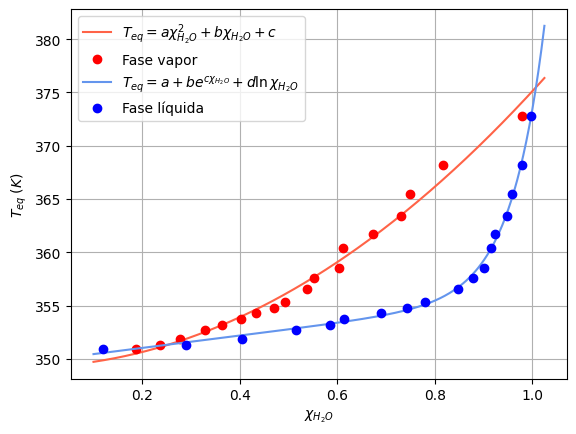
\includegraphics[width=0.65\linewidth]{ELV binario/ajustes_curva.png}
    \caption{Ajustes de las curvas de coexistencia}
    \label{fig:enter-label}
\end{figure}

En esta gráfica podemos ver claramente el comportamiento de las curvas de coexistencia, además de los puntos azeotrópicos, que se dan a fracciones molares límite, especialmente con fracciones molares de agua bajas. Estos puntos azeotrópicos se dan cuando nuestro sistema binario se comporta como si estuviera formado por una substancia pura, por lo que las curvas de las fases líquida y vapor coinciden, como se puede ver en la figura.

\subsection{Coeficientes de actividad}

Como ya introducimos en las bases teóricas, otra magnitud interesante de estudiar en nuestro sistema son los coeficientes de actividad de las fases líquidas de los diferentes componentes, para estudiar su desviación de la idealidad.  El coeficiente de actividad para la fase líquida viene dado por la expresión (\ref{gamma}), que para cada una de las componentes se puede expresar como:

\begin{equation}
    \gamma_{OH}^l(T) = \frac{\chi_{OH}^v p}{\chi_{OH}^l p_{OH}^0(T)} \quad
    \gamma_{H_2O}^l(T) = \frac{\chi_{H_2O}^v p}{\chi_{H_2O}^l p_{H_2O}^0(T)}
\end{equation}

Donde consideraremos la presión en el laboratorio, $p$, como una constante, con un valor de $1\; atm=1,01325 \cdot 10^5 \; Pa$. La incertidumbre de las fracciones molares vendrá dada por la expresión (\ref{inc_gamma}). Por otro lado, la fracción molar de etanol se calcula de forma trivial a partir de la fracción molar de agua como $\chi_{OH}^l = 1 - \chi_{H_2O}^l$, siendo $s(\chi_{OH}^l) = s(\chi_{H_2O})$. En la tabla del anexo podemos ver los datos empleados, los coeficientes de actividad y sus respectivas incertidumbres para cada una de las temperaturas de equilibrio.

Para un estudio cuantitativo del comportamiento de los coeficientes de actividad vamos a buscar una expresión analítica para $\gamma_i^l(\chi_i^l)$. Para ello vamos a ajustar nuestros los resultados obtenidos a partir de nuestros datos experimentales a funciones sencillas, a partir de ajustes no lineales.

\subsubsection{Agua}

En primer lugar, vamos a estudiar la dependencia de $\gamma_{H_2O}^l(\chi_{H_2O})$. Para ello vamos a ajustar los datos a una función del tipo:

\begin{equation}
    \gamma_{H_2O}^l = a + \frac{b}{\chi_{H_2O}^l + c}
\end{equation}

A partir de este ajuste no lineal obtuvimos los siguientes parámetros, con sus respectivas incertidumbres:

\begin{table}[h!]
    \centering
    \begin{tabular}{|c|c|}
    \hline
    $a \pm s(a) $ &  $0,726 \pm 0,036$\\ \hline
    $b\pm s(b)$ & $0,290 \pm 0,028$ \\ \hline
    $c \pm s(c)$ & $-0,0102 \pm 0,0095$\\ \hline
    \end{tabular}
    \caption{Datos del ajuste $\gamma_{H_2O}^l = a + \frac{b}{\chi_{H_2O}^l + c}$}
    \label{tab:my_label}
\end{table}

\subsubsection{Etanol}

Para el estudio de $\gamma_{OH}^l(\chi_{H_2O}^l)$ elegimos un ajuste no lineal a una función igual que la de la curva de ebullición, combinando una exponencial y un logaritmo:

\begin{equation}
    \gamma_{OH}^l = a + be^{c\chi_{H_2O}^l} + d\ln \chi_{H_2O}^l
\end{equation}

Los parámetros obtenidos a partir de este ajuste con sus respectivas incertidumbres son:

\begin{table}[h!]
    \centering
    \begin{tabular}{|c|c|}
    \hline
    $a \pm s(a) $ &  $1,48 \pm 0,19$\\ \hline
    $b\pm s(b)$ & $(1,1 \pm 1,2) \cdot 10^{-3}$ \\ \hline
    $c \pm s(c)$ & $8,1 \pm 1,2$\\ \hline
    $d \pm s(d)$ & $0,27 \pm 0,15$ \\ \hline
    \end{tabular}
    \caption{Datos del ajuste $\gamma_{OH}^l=a + be^{c\chi_{H_2O}} + d\ln \chi_{H_2O}$}
    \label{tab:my_label}
\end{table}

Cabe destacar que los ajustes empleados no fueron escogidos al azar, las funciones a ajustar tienen que verificar ciertas propiedades en las fracciones límite:

\begin{equation}
    \lim_{\chi_i^l \to 0} \gamma_i^l = \lim_{\chi_i^l \to 0} \frac{\chi_i^v p}{\chi_i^l p_i^0} = +\infty
\end{equation}

Para el ajuste de $\gamma_{H_2O}^l$ es trivial verificar esta propiedad:

\begin{equation}
    \lim_{\chi_{H_2O}^l \to 0} \gamma_{H_2O}^l =  \lim_{\chi_{H_2O}^l \to 0} a + \frac{b}{\chi_{H_2O}^l + c} = +\infty
\end{equation}

Para  verificar esta propiedad para $\gamma_{OH}^l$ debemos darnos cuenta de que $\chi_{OH}^l = 1 - \chi_{H_2O}^l$, obteniendo la siguiente equivalencia:

\begin{equation}
    \lim_{\chi_{OH}^l \to 0} \gamma_{OH}^l = \lim_{\chi_{H_2O}^l \to 1} \gamma_{OH}^l =  \lim_{\chi_{OH}^l \to 0} a + be^{c\chi_{H_2O}^l} + d \ln \chi_{H_2O}^l = +\infty
\end{equation}

Debemos notar que el resultado de este límite es $+\infty$ porque $d<0$, en caso contrario este resultado no sería válido. No o obstante, nuestro resultado para $d$ no es negativo, pero sí lo suficientemente pequeño para que represente bien el comportamiento de los coeficientes de actividad. Para obtener un resultado más satisfactorio tendríamos que contar con más puntos en el límite de $\chi_{H_2O}^l \to 0$

En la siguiente gráfica podemos ver los resultados de los ajustes no lineales, que nos permitirán interpretar mejor el comportamiento de los coeficientes de actividad:

\begin{figure}[h!]
    \centering
    \begin{subfigure}{0.49\textwidth}
        \centering
        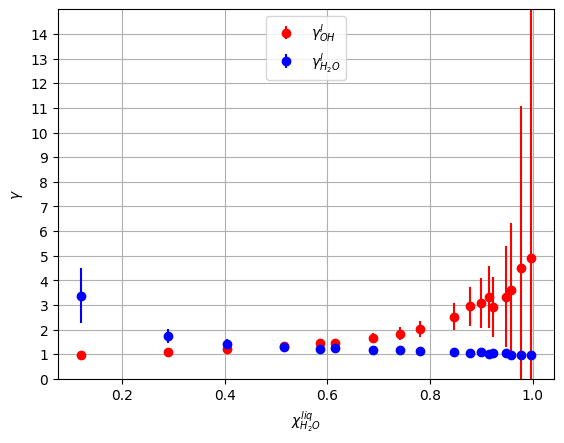
\includegraphics[width=0.95\linewidth]{ELV binario/coeficientes_inc.png}
        \subcaption{Resultados experimentales con sus incertidumbres}
    \end{subfigure}
    \begin{subfigure}{0.49\textwidth}
        \centering
        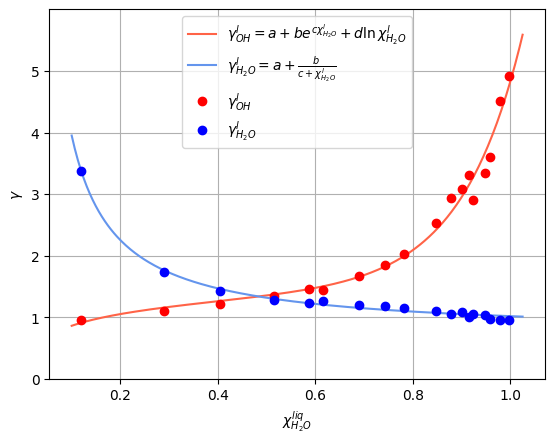
\includegraphics[width=1.05\linewidth]{ELV binario/coeficientes.png}
        \subcaption{Ajustes no lineales de $\gamma_i^l(\chi_{H_2O}^l)$}
    \end{subfigure}
    \caption{Coeficientes de actividad}
    \label{fig:enter-label}
\end{figure}

Con estas gráficas se puede entender mucho mejor el comportamiento de los coeficientes de actividad, podemos ver que a medida que la fracción molar de cada substancia se aproxima a la unidad, es decir la muestra tiende a comportarse como una substancia pura, el coeficiente de actividad tiende a 1, reflejando que esa componente se comporta dentro de la idealidad. Por otro lado, a medida que la fracción de cada uno de los componentes tiende a 0 podemos ver que el coeficiente de actividad tiende a valores cada vez más grandes, con el límite en el infinito. Esto se debe a que a fracciones molares muy bajas las moléculas de estas substancias ya no pueden ser consideradas como líquidos ideales, ya que cada vez se ven más afectadas por las interacciones con moléculas del otro componente.

Además de eso, llama la atención las altas incertidumbres que se dan en valores altos de los coeficientes de actividad, en los límites de $\chi_i^l \to 0$. Esto se debe, como ya explicamos antes, a la falta de idealidad de la substancia en estos rangos de fracciones molares muy bajas.

\newpage

\subsection{Entalpía libre de exceso}

Como ya hemos introducido antes, otra magnitud interesante para estudiar la idealidad del sistema es la entalpía libre de exceso, que refleja la diferencia entre la entalpía libre del sistema y la del sistema si se comportara de forma ideal. Esta magnitud viene reflejada por la Ec.\ref{delta_g}. En la tabla del anexo podemos ver los resultados obtenidos con sus incertidumbres.

A partir de estos datos y de igual forma que con los coeficientes de actividad, vamos a buscar una expresión analítica para $\Delta g^{E}(\chi_{H_2O}^l)$. Para ello podemos aproximar nuestros datos a un polinomio, en nuestro caso escogimos un polinomio de grado 4, del tipo:

\begin{equation}
    \Delta g^{E} = a\chi_{H_2O}^4 + b\chi_{H_2O}^3 + c\chi_{H_2O}^2 + d\chi_{H_2O} + e
\end{equation}

En la siguiente tabla podemos ver los parámetros obtenidos a partir del ajuste, así como sus respectivas incertidumbres:

\begin{table}[h!]
    \centering
    \begin{tabular}{|c|c|}
    \hline
    $a \pm s(a) \;(kJ/mol)$ &  $-4,59 \pm 0,90$\\ \hline
    $b\pm s(b) \; (kJ/mol)$ & $9,0 \pm 2,1$ \\ \hline
    $c \pm s(c) \; (kJ/mol)$ & $-6,5 \pm 1,6$\\ \hline
    $d \pm s(d) \; (kJ/mol)$ & $2,13 \pm 0,50$ \\ \hline
    $e \pm s(e) \; (kJ/mol)$ & $-0,104 \pm 0,047$ \\ \hline
    \end{tabular}
    \caption{Datos del ajuste $\Delta g^{E} = a\chi_{H_2O}^4 + b\chi_{H_2O}^3 + c\chi_{H_2O}^2 + d\chi_{H_2O} + e$}
    \label{tab:my_label}
\end{table}

Una vez hecho el ajuste, podemos representar gráficamente los resultados obtenidos, para poder extraer conclusiones respecto a la idealidad del sistema:

\newpage

\begin{figure}[h!]
    \centering
    \begin{subfigure}{0.49\textwidth}
        \centering
        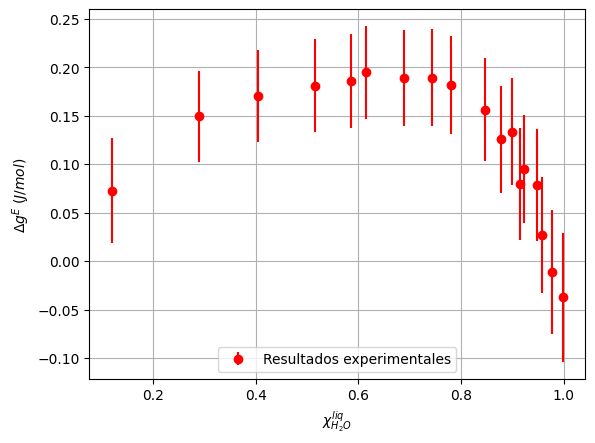
\includegraphics[width=1.\linewidth]{ELV binario/entalpia_inc.png}
        \subcaption{Resultados experimentales con sus incertidumbres}
    \end{subfigure}
    \begin{subfigure}{0.49\textwidth}
        \centering
        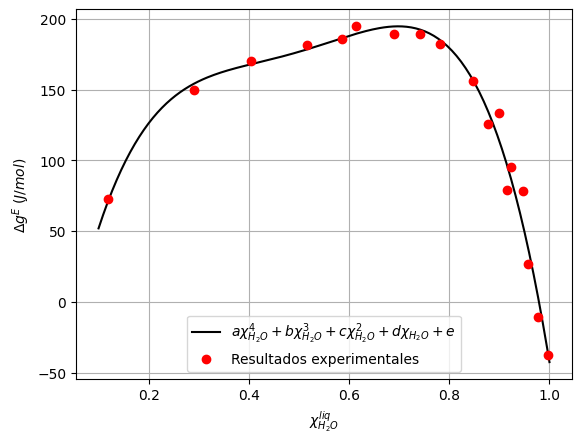
\includegraphics[width=1.05\linewidth]{ELV binario/entalpia.png}
        \subcaption{Ajuste polinómico}
    \end{subfigure}
    \caption{Entalpías libres de exceso}
    \label{fig:enter-label}
\end{figure}

Podemos observar que los valores de las entalpías libres de exceso tienden a anularse en los extremos, donde la disolución presenta un comportamiento más ideal, ya que tiende a comportarse como una substancia pura. Por el medio vemos que las entalpías de exceso aumentan notablemente, ya que nuestro sistema se comporta como una disolución no ideal. Además de eso, resulta destacable las altas incertidumbres que presentan todos los valores de las entalpías libres de exceso. Esto es algo que podríamos prever, ya que las incertidumbres de las entalpías libres derivan de magnitudes a las cuales ya hemos aplicado propagación de incertidumbres, como los $\gamma_i$ y las $\chi_i$. Todas estas incertidumbres acumuladas hacen que la incertidumbre final tenga valores bastante altos, llegando incluso a superar al resultado experimental en muchas ocasiones. No obstante, esto no impide que se pueda observar el comportamiento esperado para esta magnitud, que refleja claramente la idealidad que presentan las muestras que tienden a substancias puras.


\subsection{Presiones de Raoult}

Para finalizar, presentaremos una última forma de estudiar la idealidad de nuestro sistema, mediante la ley de Raoult y el estudio de la presión que ejerce cada componente. Para ello, como ya hemos introducido antes, emplearemos las expresiones deducidas durante la práctica de ELV simple para $p_i^0(T)$ para cada una de las substancias. Estas expresiones nos permitirán obtener la curva $p^R_i$ para cada una de las substancias, a partir de ahí no tendremos más que sumar las presiones para obtener la presión total predicha por la ley de Raoult, que compararemos con la presión atmosférica en el laboratorio, que consideraremos de $1\; atm = 1,01325 \;Bar$, como ya mencionamos. En la tabla del anexo podemos ver los resultados obtenidos con sus respectivas incertidumbres.

A partir de estos datos vamos a buscar una expresión analítica para las diferentes presiones de Raoult que ejercen el agua, el etanol y el sistema binario de agua y etanol.

\subsubsection{Agua}

En primer lugar vamos a obtener una expresión analítica para $p_{H_2O}^R(\chi_{H_2O}^l)$, para ello vamos a aproximar nuestros datos por un polinomio de cuarto grado, ya que presentan una tendencia algo compleja:

\begin{equation}
    p^R_{H_2O}(\chi_{H_2O}^l) = a \chi_{H_2O}^4 + b \chi_{H_2O}^3 + c \chi_{H_2O}^2 + d\chi_{H_2O} + e  
\end{equation}

Los parámetros obtenidos a partir de nuestro ajuste con sus respectivas incertidumbres son:

\begin{table}[h!]
    \centering
    \begin{tabular}{|c|c|}
    \hline
    $a \pm s(a) \;(Bar)$ &  $13,0 \pm 2,3$\\ \hline
    $b\pm s(b) \; (Bar)$ & $-25,7 \pm 5,3$ \\ \hline
    $c \pm s(c) \; (Bar)$ & $17,3 \pm 4,2$\\ \hline
    $d \pm s(d) \; (Bar)$ & $-4,0 \pm 1,3$ \\ \hline
    $e \pm s(e) \; (Bar)$ & $0,33 \pm 0,12$ \\ \hline
    \end{tabular}
    \caption{Datos del ajuste de $p^R_{H_2O}$}
    \label{tab:my_label}
\end{table}

\subsubsection{Etanol}

Por otro lado, los datos del etanol presentan una tendencia mucho más simple, pudiendo realizar una buena modelización de los datos con una regresión lineal a una recta del tipo $y=a+bx$ para obtener la expresión $p_{OH}^R(\chi_{H_2O}^l)$. Los parámetros obtenidos a partir de la regresión fueron:

\begin{table}[h!]
\centering
\begin{tabular}{|c|c|}
\hline
$a \pm s(a) \;(Bar)$ &  $0,9887 \pm 0,0093$\\ \hline
$b \pm s(b) \; (Bar)$ &  $-0,954 \pm 0,012$\\ \hline
r            &  $-0,998$\\ \hline
\end{tabular}
\caption{Datos de la regresión $p^R_{OH} = a + b\chi_{H_2O}^l$}
\label{tab:my-table}
\end{table}

\subsubsection{Sistema binario etanol-agua}

Por último, vamos a obtener una expresión analítica para $p_T^R(\chi_{H_2O}^l)$, que no es más que una expresión analítica para la suma de las presiones. Para ello vamos a aproximar nuestros datos a un polinomio de cuarto grado, como era de esperar teniendo en cuenta los ajustes anteriores, otro polinomio de grado cuatro y un término lineal. Los parámetros obtenidos con sus respectivas incertidumbres son:

\begin{table}[h!]
    \centering
    \begin{tabular}{|c|c|}
    \hline
    $a \pm s(a) \;(Bar)$ &  $12,5 \pm 2,0$\\ \hline
    $b\pm s(b) \; (Bar)$ & $-25,0 \pm 4,7$ \\ \hline
    $c \pm s(c) \; (Bar)$ & $17,0 \pm 3,7$\\ \hline
    $d \pm s(d) \; (Bar)$ & $-4,8 \pm 1,1$ \\ \hline
    $e \pm s(e) \; (Bar)$ & $1,29 \pm 0,11$ \\ \hline
    \end{tabular}
    \caption{Datos del ajuste de $p^R_{T}$}
    \label{tab:my_label}
\end{table}

En la siguiente figura podemos ver representados todos los datos de la presiones obtenidos con la ley de Raoult, sus respectivos ajustes, así como el valor que tomamos de referencia de la presión atmosférica del laboratorio:

\begin{figure}[h!]
    \centering
    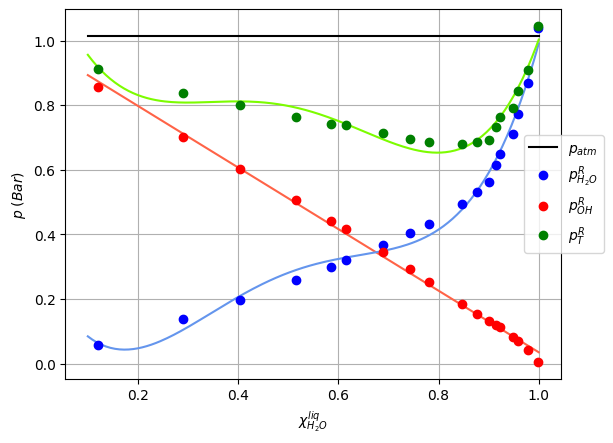
\includegraphics[width=0.75\linewidth]{ELV binario/raoult.png}
    \caption{Presiones de Raoult}
    \label{fig:enter-label}
\end{figure}

Tras ver una representación gráfica de los resultados resulta mucho más sencillo darles una interpretación física. Podemos ver claramente que a medida que a medida que las muestras tienden a ser más puras el sistema tiende al comportamiento ideal. Además de eso, debemos destacar que se produce una desviación positiva de la ley de Raoult, ya que la presión de la mezcla, que se corresponde con la presión del laboratorio, es mayor que la presión de Raoult. Este resultado era esperado, ya que las desviaciones positivas se dan en sistemas donde las fuerzas cohesivas entre moléculas de la misma especie son mayores que las fuerzas adhesivas entre moléculas diferentes, algo esperado en un sistema formado por moléculas polares como el etanol y el agua, que presentan enlaces por puentes de hidrógeno.

\section{Conclusiones}

Como conclusión, podemos ver que los resultados del experimento se corresponden con lo esperado. Las curvas de coexistencia obtenidas son un buen reflejo de estos resultados, ofreciendo una representación del comportamiento de nuestro sistema binario en la situación de equilibrio líquido-vapor en función de la composición del propio sistema.

Además de eso, realizamos un estudio de la idealidad del sistema, introduciendo conceptos como los coeficientes de actividad de la fase líquida, las variaciones de entalpía libre de exceso o las presiones de Raoult. Todas estas magnitudes nos dan diferentes perspectivas sobre la idealidad del sistema empleando diferentes enfoques. Los coeficientes de actividad reflejan desde un punto de vista de las interacciones moleculares que la idealidad se da en sistemas que tienden a ser muestras puras. Por otro lado las entalpías libres de exceso corroboran esto desde un punto de vista energético, así como las presiones de Raoult lo hacen desde un estudio en la magnitud intensiva por excelencia para caracterizar a un fluido, como es la presión. Con todo, podemos concluir que los resultados fueron satisfactorios y que el comportamiento de nuestro sistema binario queda bien reflejado con nuestros resultados experimentales.

\section{Bibliografía}

\begin{itemize}
    \item Guión de prácticas
    \item \textit{NIST Chemistry WebBook}. https://webbook.nist.gov/chemistry/
    \item \textit{Equilibrio vapor-líquido}. https://es.wikipedia.org/wiki/Equilibrio\_vapor-liquido
\end{itemize}

\newpage

\section{Anexo: Datos experimentales}

\begin{table}[h!]
\centering
\begin{tabular}{|c|c|c|c|c|c|c|}
\hline
$T_{eq}\; (K)$               & 372,8  & 368,2  & 365,5  & 363,4  & 361,7  & 360,4  \\ \hline
$\rho_v\; (g/cm^3)$          & 0,9885 & 0,9371 & 0,9174 & 0,9128 & 0,8978 & 0,8826 \\ \hline
$\chi_{H_2O}^v$             & 0,979  & 0,818  & 0,749  & 0,732  & 0,674  & 0,611  \\ \hline
$s(\chi_{H_2O}^v)$          & 0,032  & 0,031  & 0,031  & 0,031  & 0,031  & 0,030  \\ \hline
$\chi_{OH}^v$               & 0,021  & 0,182  & 0,251  & 0,268  & 0,326  & 0,389  \\ \hline
$\rho_l\; (g/cm^3)$          & 0,9952 & 0,9883 & 0,9815 & 0,9781 & 0,9697 & 0,9673 \\ \hline
$\chi_{H_2O}^l$             & 0,998  & 0,978  & 0,958  & 0,948  & 0,923  & 0,915  \\ \hline
$s(\chi_{H_2O}^l)$          & 0,032  & 0,032  & 0,031  & 0,031  & 0,031  & 0,031  \\ \hline
$\chi_{OH}^l$               & 0,002  & 0,022  & 0,042  & 0,052  & 0,077  & 0,085  \\ \hline
$p_{H_2O}^0 \;(Bar)$         & 1,043  & 0,889  & 0,807  & 0,749  & 0,704  & 0,671  \\ \hline
$s(p_{H_2O}^0) \;(Bar)$      & 0,032  & 0,027  & 0,025  & 0,023  & 0,022  & 0,021  \\ \hline
$\gamma_{H_2O}^l$            & 2,196  & 1,865  & 1,692  & 1,567  & 1,471  & 1,401  \\ \hline
$s(\gamma_{H_2O}^l)$         & 0,095  & 0,081  & 0,074  & 0,069  & 0,065  & 0,062  \\ \hline
$p_{OH}^0 \;(Bar)$           & 0,953  & 0,953  & 0,981  & 1,045  & 1,052  & 1,008  \\ \hline
$s(p_{OH}^0) \;(Bar)$        & 0,052  & 0,056  & 0,060  & 0,064  & 0,068  & 0,068  \\ \hline
$\gamma_{OH}^l$              & 5      & 4,5    & 3,6    & 3,3    & 2,9    & 3,3    \\ \hline
$s(\gamma_{OH}^l)$           & 78     & 6,6    & 2,7    & 2,1    & 1,2    & 1,3    \\ \hline
$\Delta g^{E} \; (J/mol)$    & -37    & -11    & 27     & 78     & 95     & 79     \\ \hline
$s(\Delta g^{E}) \; (J/mol)$ & 67     & 64     & 60     & 58     & 56     & 58     \\ \hline
$p_{H_2O}^R \;(Bar)$         & 1,041  & 0,869  & 0,774  & 0,710  & 0,649  & 0,614  \\ \hline
$s(p_{H_2O}^R) \;(Bar)$      & 0,046  & 0,039  & 0,035  & 0,032  & 0,030  & 0,028  \\ \hline
$p_{OH}^R \;(Bar)$           & 0,004  & 0,041  & 0,071  & 0,081  & 0,114  & 0,119  \\ \hline
$s(p_{OH}^R) \;(Bar)$        & 0,069  & 0,059  & 0,053  & 0,049  & 0,046  & 0,044  \\ \hline
$p_{T}^R \;(Bar)$            & 1,045  & 0,910  & 0,844  & 0,791  & 0,763  & 0,733  \\ \hline
$s(p_{T}^R) \;(Bar)$         & 0,083  & 0,070  & 0,064  & 0,059  & 0,055  & 0,053  \\ \hline
\end{tabular}
\caption{Datos experimentales 1}
\label{tab:my-table}
\end{table}

\newpage

\begin{table}[h!]
\centering
\begin{tabular}{|c|c|c|c|c|c|c|}
\hline
$T_{eq}\; (K)$               & 358,5  & 357,6  & 356,6  & 355,3  & 354,8  & 354,3  \\ \hline
$\rho_v\; (g/cm^3)$          & 0,881  & 0,8695 & 0,8663 & 0,8571 & 0,8527 & 0,846  \\ \hline
$\chi_{H_2O}^v$             & 0,604  & 0,553  & 0,538  & 0,492  & 0,470  & 0,433  \\ \hline
$s(\chi_{H_2O}^v)$          & 0,030  & 0,030  & 0,030  & 0,030  & 0,030  & 0,030  \\ \hline
$\chi_{OH}^v$               & 0,396  & 0,447  & 0,462  & 0,508  & 0,530  & 0,567  \\ \hline
$\rho_l\; (g/cm^3)$          & 0,9624 & 0,9553 & 0,946  & 0,9264 & 0,9157 & 0,9016 \\ \hline
$\chi_{H_2O}^l$             & 0,900  & 0,878  & 0,848  & 0,781  & 0,742  & 0,689  \\ \hline
$s(\chi_{H_2O}^l)$          & 0,031  & 0,031  & 0,031  & 0,031  & 0,031  & 0,031  \\ \hline
$\chi_{OH}^l$               & 0,100  & 0,122  & 0,152  & 0,219  & 0,258  & 0,311  \\ \hline
$p_{H_2O}^0 \;(Bar)$         & 0,626  & 0,605  & 0,583  & 0,555  & 0,544  & 0,534  \\ \hline
$s(p_{H_2O}^0) \;(Bar)$      & 0,019  & 0,019  & 0,018  & 0,017  & 0,017  & 0,017  \\ \hline
$\gamma_{H_2O}^l$            & 1,304  & 1,261  & 1,213  & 1,154  & 1,132  & 1,110  \\ \hline
$s(\gamma_{H_2O}^l)$         & 0,058  & 0,056  & 0,054  & 0,051  & 0,050  & 0,049  \\ \hline
$p_{OH}^0 \;(Bar)$           & 1,088  & 1,055  & 1,103  & 1,152  & 1,177  & 1,19   \\ \hline
$s(p_{OH}^0) \;(Bar)$        & 0,074  & 0,076  & 0,081  & 0,091  & 0,096  & 0,10   \\ \hline
$\gamma_{OH}^l$              & 3,1    & 2,94   & 2,53   & 2,03   & 1,84   & 1,66   \\ \hline
$s(\gamma_{OH}^l)$           & 1,0    & 0,79   & 0,55   & 0,32   & 0,26   & 0,20   \\ \hline
$\Delta g^{E} \; (J/mol)$    & 134    & 126    & 156    & 182    & 190    & 189    \\ \hline
$s(\Delta g^{E}) \; (J/mol)$ & 55     & 55     & 53     & 51     & 50     & 49     \\ \hline
$p_{H_2O}^R \;(Bar)$         & 0,563  & 0,531  & 0,494  & 0,433  & 0,404  & 0,368  \\ \hline
$s(p_{H_2O}^R) \;(Bar)$      & 0,026  & 0,025  & 0,024  & 0,022  & 0,021  & 0,020  \\ \hline
$p_{OH}^R \;(Bar)$           & 0,130  & 0,154  & 0,185  & 0,253  & 0,292  & 0,345  \\ \hline
$s(p_{OH}^R) \;(Bar)$        & 0,041  & 0,040  & 0,039  & 0,037  & 0,037  & 0,037  \\ \hline
$p_{T}^R \;(Bar)$            & 0,693  & 0,685  & 0,679  & 0,686  & 0,696  & 0,713  \\ \hline
$s(p_{T}^R) \;(Bar)$         & 0,049  & 0,047  & 0,045  & 0,043  & 0,043  & 0,042  \\ \hline
\end{tabular}
\caption{Datos experimentales 2}
\label{tab:my-table}
\end{table}

\newpage

\begin{table}[]
\centering
\begin{tabular}{|c|c|c|c|c|c|c|}
\hline
$T_{eq}\; (K)$               & 353,7  & 353,2  & 352,7  & 351,9  & 351,3  & 350,9  \\ \hline
$\rho_v\; (g/cm^3)$          & 0,8407 & 0,8344 & 0,829  & 0,8218 & 0,8168 & 0,8112 \\ \hline
$\chi_{H_2O}^v$             & 0,403  & 0,364  & 0,329  & 0,277  & 0,237  & 0,187  \\ \hline
$s(\chi_{H_2O}^v)$          & 0,030  & 0,029  & 0,029  & 0,030  & 0,030  & 0,031  \\ \hline
$\chi_{OH}^v$               & 0,597  & 0,636  & 0,671  & 0,723  & 0,763  & 0,813  \\ \hline
$\rho_l\; (g/cm^3)$          & 0,8834 & 0,8768 & 0,8618 & 0,8409 & 0,8235 & 0,8049 \\ \hline
$\chi_{H_2O}^l$             & 0,615  & 0,586  & 0,516  & 0,404  & 0,290  & 0,119  \\ \hline
$s(\chi_{H_2O}^l)$          & 0,030  & 0,030  & 0,030  & 0,030  & 0,030  & 0,034  \\ \hline
$\chi_{OH}^l$               & 0,385  & 0,414  & 0,484  & 0,596  & 0,710  & 0,881  \\ \hline
$p_{H_2O}^0 \;(Bar)$         & 0,522  & 0,512  & 0,502  & 0,487  & 0,476  & 0,469  \\ \hline
$s(p_{H_2O}^0) \;(Bar)$      & 0,016  & 0,016  & 0,016  & 0,015  & 0,015  & 0,015  \\ \hline
$\gamma_{H_2O}^l$            & 1,085  & 1,064  & 1,043  & 1,011  & 0,988  & 0,972  \\ \hline
$s(\gamma_{H_2O}^l)$         & 0,048  & 0,047  & 0,047  & 0,045  & 0,044  & 0,044  \\ \hline
$p_{OH}^0 \;(Bar)$           & 1,27   & 1,23   & 1,29   & 1,43   & 1,74   & 3,4    \\ \hline
$s(p_{OH}^0) \;(Bar)$        & 0,12   & 0,12   & 0,14   & 0,19   & 0,29   & 1,1    \\ \hline
$\gamma_{OH}^l$              & 1,45   & 1,46   & 1,35   & 1,216  & 1,102  & 0,963  \\ \hline
$s(\gamma_{OH}^l)$           & 0,15   & 0,14   & 0,12   & 0,095  & 0,080  & 0,067  \\ \hline
$\Delta g^{E} \; (J/mol)$    & 195    & 186    & 181    & 170    & 150    & 73     \\ \hline
$s(\Delta g^{E}) \; (J/mol)$ & 48     & 48     & 48     & 47     & 47     & 54     \\ \hline
$p_{H_2O}^R \;(Bar)$         & 0,321  & 0,300  & 0,259  & 0,197  & 0,138  & 0,056  \\ \hline
$s(p_{H_2O}^R) \;(Bar)$      & 0,019  & 0,018  & 0,017  & 0,016  & 0,015  & 0,016  \\ \hline
$p_{OH}^R \;(Bar)$           & 0,418  & 0,441  & 0,505  & 0,603  & 0,701  & 0,856  \\ \hline
$s(p_{OH}^R) \;(Bar)$        & 0,038  & 0,038  & 0,039  & 0,040  & 0,043  & 0,050  \\ \hline
$p_{T}^R \;(Bar)$            & 0,739  & 0,741  & 0,764  & 0,800  & 0,839  & 0,912  \\ \hline
$s(p_{T}^R) \;(Bar)$         & 0,042  & 0,042  & 0,042  & 0,043  & 0,045  & 0,053  \\ \hline
\end{tabular}
\caption{Datos experimentales 3}
\label{tab:my-table}
\end{table}

\end{document}